
\iffalse
\begin{figure}
    \centering
    \includegraphics[width=12cm]{../figures/blip_bbh_runs_two_panel_comparison.pdf}
    \caption{Glitch panel comparison}
    \label{fig:qscan_null}
\end{figure}
\fi

\begin{table}[h!]
    \centering
    \renewcommand{\arraystretch}{1.2}
    \begin{tabular}{p{0.45\textwidth}|p{0.45\textwidth}}
    \toprule
    \textbf{LIGO-Virgo interferometers} & \textbf{Third-generation interferometers} \\
    \midrule
    \begin{enumerate}[leftmargin=*, label=\arabic*.]
        \item Detection rate of $\mathcal{O}(1)$ signal per week
        \item A GW signal is in-band for $\mathcal{O}(1)$ second to $\mathcal{O}(1)$ minute. Therefore, nearly every segment of data contains only noise. 
        \item Glitch rate of $\mathcal{O}(1)$ per minute across three observation runs. 
        \item \textit{Almost} all glitches occur in isolation due to smaller in-band duration and smaller detection rate of GW signals. 
        \item Almost all glitches can be vetoed without incurring significant loss of GW signals. 
    \end{enumerate}
    &
    \begin{enumerate}[leftmargin=*, label=\arabic*.]
        \item Detection rate of $\mathcal{O}(1)$ signal per minute
        \item A GW signal is in-band for $\mathcal{O}(1)$ minute to $\mathcal{O}(1)$ hour. Therefore, nearly every segment of data is expected to contain a signal. 
        \item Glitch rate is unknown. Let's assume same as LIGO-Virgo interferometers.
        \item \textit{Almost} all glitches will overlap with a GW signal due to larger in-band duration and larger detection rate. 
        \item Very few glitches may be vetoed without losing GW signals. 
    \end{enumerate}
    \\
    \bottomrule
    \end{tabular}
    \caption{Problem posed by glitches in LIGO-Virgo interferometers versus third-generation interferometers.}
    \label{tab:glitch_diff}
\end{table}
When occuring in the vicinity of a GW signal, glitches (or transient noises) can corrupt the signal. Signal-overlapping glitches need to be carefully removed before measuring the GW source parameters. Such glitches are problematic for the LIGO-Virgo interferometers as nearly $\sim 20$ out of 90 confident detection across three observation runs required some form of glitch mitigation and this number will keep growing as we collect more data. 




While glitch mitigation is an active area of research for current detectors, it is yet to recieve similar attention in the context of 3G-detectors. In Table~\ref{tab:glitch_diff}, we compare the problem posed by glitches for the LIGO-Virgo and the 3G interferometers. Glitches could turn out to be a major bottelneck in transitioning to the precision science era. In this chapter, we introduce the \texttt{nijntje} -- a null stream inspired noise transient elimination framework to tackle this problem.   

\section{The null stream of the Einstein Telescope}
The null stream is a linear combination of the data from a network of interferometers such that the GW signal cancels out. For the triangular geometry of the Einstein Telescope this linear combination is simply the sum of the data from three detectors. 

\begin{equation}
    \vec{d}_i = F_{+, i} h_+ + F_{\times, i} h_{\times}
\end{equation}

[Place holder figure of null stream antenna pattern functions]

\section{A null-stream inspired noise transient elimination (\texttt{nijntje}) framework}
\begin{figure}
    \centering
    \includegraphics[width=16cm]{../figures/assemble_nijntje.pdf}
    \caption{The blue box outlines the workflow of \texttt{nijntje} algorithm. \textit{Step 1}: Construct the null stream by summing the strain data from three interferometers. \textit{Step 2}: Using the null stream data and an RJMCMC method, perform an unmodelled reconstruction of the glitch timeseries. \textit{Step 3}: Find the glitch timeseries which corresponds to the median of the posterior samples and subtract it from $\mathrm{ET}_1$ frame. \textit{Step 4} (Optional): Perform parameter estimation using the cleaned data from $\mathrm{ET}_1$, and the existing data from $\mathrm{ET}_2$ and $\mathrm{ET}_3$ to verify the accuracy.}
    \label{fig:nijntje_chart}
\end{figure}

\section{Comparison between the triangle and L-shpaed interferometer}
\begin{figure}
    \centering
    \includegraphics[width=10cm]{../figures/et2l_delta_glitch_overlap_glitch_master.pdf}
    \caption{Glitch overlap}
    \label{fig:glitch_overlap}
\end{figure}

\begin{figure}
    \centering
    \includegraphics[width=10cm]{../figures/newsnr_mismatch_comparison.pdf}
    \caption{Mismatch}
    \label{fig:mismatch}
\end{figure}

\begin{figure}
    \centering
    \includegraphics[width=16cm]{../figures/newsnr_fig_4.pdf}
    \caption{Mass Distance Sky}
    \label{fig:delta_zero}
\end{figure}

\begin{figure}
    \centering
    \includegraphics[width=10cm]{../figures/newsnr_rank_10_single_block_percentile_parameters_short.pdf}
    \caption{Confidence interval}
    \label{fig:trend_delta}
\end{figure}

\section{Caveats}


